\title{How to hide data in dithering patterns}

In this note we describe a simple method for encoding arbitrary data in
dithered binary images.
The density is about 0.25 bits per pixel in non-saturated
regions, and zero bits in saturated regions.
Unless the encoded data has some pattern, the encoding is not visible.

\section{Description of the method}

Sometimes you need to represent gray-scale data by black and white pixels.
The simplest technique is~\emph{random dithering}, where you throw a random
binary pixel with the probability of being white determined by the gray
level.  Random dithering is trivial to implement, but it loses a lot of
resolution.  A better technique is~\emph{error diffusion}, where you traverse
the pixels in a certain order order and select the black or white value that
minimizes the ongoing average error.  Notice that this depends on the order
of traversal.  For uniform regions it tends to produce visible patterns, and
this can be avoided by traversing the pixels in a more or less irregular way
(for example, a Hilbert curve is often used).


\begin{tabular}{ccc}
	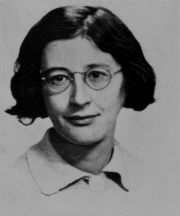
\includegraphics{i/psimone.png} &
	\href{z-psimone-random.png}{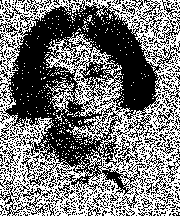
\includegraphics{psimone-random.png}} &
	\href{z-psimone-errdif.png}{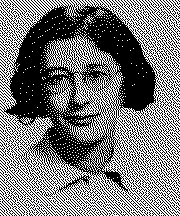
\includegraphics{psimone-errdif.png}} \\
	gray-scale &
	random &
	error diffusion
\end{tabular}
%SCRIPT plambda i/psimone.png 'randu 255 * > 255 *' -o psimone-random.png
%SCRIPT dither i/psimone.png psimone-errdif.png

%By preprocessing the image before dithering (gamma correction or retinex), we
%can control a bit the final aspect.

Since there is a lot of choice when dithering an image, we can encode a lot
of information in these choices.  Assuming that we will be able to recover
the binary image exactly, the simplest way to encode the data is to have a
{\bf table of patterns} such as this:

\begin{tabular}{lcccccccccccccccc}
	pattern &
	
\includegraphics{pat_0.png} &
	
\includegraphics{pat_1.png} &
	
\includegraphics{pat_2.png} &
	
\includegraphics{pat_3.png} &
	
\includegraphics{pat_4.png} &
	
\includegraphics{pat_5.png} &
	
\includegraphics{pat_6.png} &
	
\includegraphics{pat_7.png} &
	
\includegraphics{pat_8.png} &
	
\includegraphics{pat_9.png} &
	
\includegraphics{pat_10.png} &
	
\includegraphics{pat_11.png} &
	
\includegraphics{pat_12.png} &
	
\includegraphics{pat_13.png} &
	
\includegraphics{pat_14.png} &
	
\includegraphics{pat_15.png} \\
	index &
	0 & 1 & 2 & 3 & 4 & 5 & 6 & 7 & 8 & 9 & 10 & 11 & 12 & 13 & 14 & 15 \\
	intensity &
	0 & 1 & 1 & 2 & 1 & 2 & 2 & 3 & 1 & 2 &  2 &  3 &  2 &  3 &  3 &  4 \\
	group &
	$-$ & $a_0$ & $a_1$ & $-$ & $b_0$ & $c_0$ & $c_1$ & $d_0$ &
	$b_1$ & $e_0$ & $e_1$ & $d_1$ & $-$ & $f_0$ & $f_1$ & $-$ \\
\end{tabular}


%SCRIPT printf 'P2\n2 2\n1\n0 0 0 0\n'|plambda '200 *'|ntiply 16 - pat_0.png
%SCRIPT printf 'P2\n2 2\n1\n0 0 0 1\n'|plambda '200 *'|ntiply 16 - pat_1.png
%SCRIPT printf 'P2\n2 2\n1\n0 0 1 0\n'|plambda '200 *'|ntiply 16 - pat_2.png
%SCRIPT printf 'P2\n2 2\n1\n0 0 1 1\n'|plambda '200 *'|ntiply 16 - pat_3.png
%SCRIPT printf 'P2\n2 2\n1\n0 1 0 0\n'|plambda '200 *'|ntiply 16 - pat_4.png
%SCRIPT printf 'P2\n2 2\n1\n0 1 0 1\n'|plambda '200 *'|ntiply 16 - pat_5.png
%SCRIPT printf 'P2\n2 2\n1\n0 1 1 0\n'|plambda '200 *'|ntiply 16 - pat_6.png
%SCRIPT printf 'P2\n2 2\n1\n0 1 1 1\n'|plambda '200 *'|ntiply 16 - pat_7.png
%SCRIPT printf 'P2\n2 2\n1\n1 0 0 0\n'|plambda '200 *'|ntiply 16 - pat_8.png
%SCRIPT printf 'P2\n2 2\n1\n1 0 0 1\n'|plambda '200 *'|ntiply 16 - pat_9.png
%SCRIPT printf 'P2\n2 2\n1\n1 0 1 0\n'|plambda '200 *'|ntiply 16 - pat_10.png
%SCRIPT printf 'P2\n2 2\n1\n1 0 1 1\n'|plambda '200 *'|ntiply 16 - pat_11.png
%SCRIPT printf 'P2\n2 2\n1\n0 0 0 0\n'|plambda '200 *'|ntiply 16 - pat_0.png
%SCRIPT printf 'P2\n2 2\n1\n1 1 0 0\n'|plambda '200 *'|ntiply 16 - pat_12.png
%SCRIPT printf 'P2\n2 2\n1\n1 1 0 1\n'|plambda '200 *'|ntiply 16 - pat_13.png
%SCRIPT printf 'P2\n2 2\n1\n1 1 1 0\n'|plambda '200 *'|ntiply 16 - pat_14.png
%SCRIPT printf 'P2\n2 2\n1\n1 1 1 1\n'|plambda '200 *'|ntiply 16 - pat_15.png

A binary image is thus divided in~$2\times2$ cells, and each cell is identified
with one of the patterns of the table (cells marked with~``$-$'' are not used).
Then the pairs of patterns~$x_0$ and~$x_1$, which have always the same
intensity, are considered equivalent and each of them is used to encode a bit
of information, losing the original pattern.

The~\emph{carrying bit content} of a binary image is defined as the number
of~$2\times2$ cells that match a valid pattern in this table.
Notice that saturated regions (either black or white) can not encode any
information, so that it is better to avoid them as much as possible.
They can be avoided, for example, by applying a retinex-like transform in the
input image, before dithering.

\begin{tabular}{l|cccc}
	&
	original &
	$\gamma=0.5$ &
	$\gamma=2$ &
	retinex \\
	\hline
	gray &
	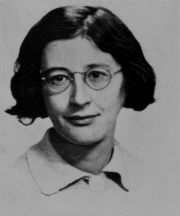
\includegraphics{i/psimone.png} &
	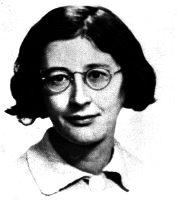
\includegraphics{psimone-gam.png} &
	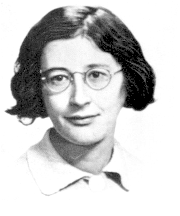
\includegraphics{psimone-ugam.png} &
	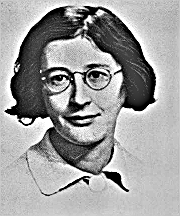
\includegraphics{psimone-ret.png} \\
	binary &
	\href{z-psimone-errdif.png}{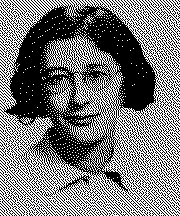
\includegraphics{psimone-errdif.png}}  &
	\href{z-psimone-gamdit.png}{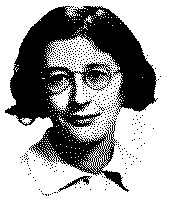
\includegraphics{psimone-gamdit.png}}  &
	\href{z-psimone-ugamdit.png}{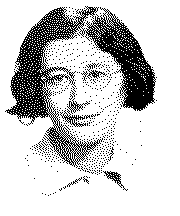
\includegraphics{psimone-ugamdit.png}} &
	\href{z-psimone-retdit.png}{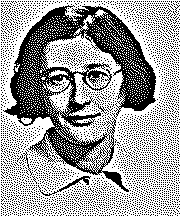
\includegraphics{psimone-retdit.png}}  \\
	bytes &
	\input{berrdit.txt} &
	\input{bgamdit.txt} &
	\input{bugamdit.txt} &
	\input{bretdit.txt} \\
	bytes(2) &
	\input{b2errdit.txt} &
	\input{b2gamdit.txt} &
	\input{b2ugamdit.txt} &
	\input{b2retdit.txt} \\
\end{tabular}
%SCRIPT qeasy 0 160 i/psimone.png psimone-sat.png
%SCRIPT plambda i/psimone.png '160 / 2 ^ 255 *' -o psimone-gam.png
%SCRIPT plambda i/psimone.png '160 / 0.5 ^ 255 *' -o psimone-ugam.png
%SCRIPT plambda i/psimone.png 'x,l -1 *'|blur z 0.2|qauto - psimone-ret.png
%SCRIPT dither psimone-sat.png psimone-satdit.png
%SCRIPT dither psimone-gam.png psimone-gamdit.png
%SCRIPT dither psimone-ugam.png psimone-ugamdit.png
%SCRIPT dither psimone-ret.png psimone-retdit.png
%SCRIPT mdither count psimone-errdif.png  | cut -d' ' -f 3 > berrdit.txt
%SCRIPT mdither count psimone-gamdit.png  | cut -d' ' -f 3 > bgamdit.txt
%SCRIPT mdither count psimone-ugamdit.png | cut -d' ' -f 3 > bugamdit.txt
%SCRIPT mdither count psimone-retdit.png  | cut -d' ' -f 3 > bretdit.txt
%SCRIPT mdither2 count psimone-errdif.png  | cut -d' ' -f 3 > b2errdit.txt
%SCRIPT mdither2 count psimone-gamdit.png  | cut -d' ' -f 3 > b2gamdit.txt
%SCRIPT mdither2 count psimone-ugamdit.png | cut -d' ' -f 3 > b2ugamdit.txt
%SCRIPT mdither2 count psimone-retdit.png  | cut -d' ' -f 3 > b2retdit.txt

The following figure shows the effect of the actual encoding.  We encode a
stream of random bits, and a stream of zero bits.  Notice that the stream of
zeros introduces a visible pattern in the image.  To avoid these patterns,
the data to be encoded must have a uniform distribution (for example, by
compressing it).

\begin{tabular}{ccc}
	\href{z-psimone-retdit.png}{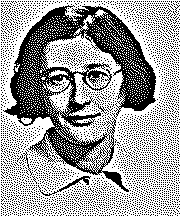
\includegraphics{psimone-retdit.png}}&
	\href{z-psimone-retditR.png}{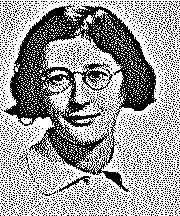
\includegraphics{psimone-retditR.png}}&
	\href{z-psimone-retditZ.png}{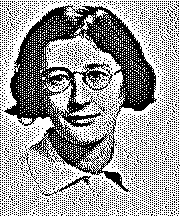
\includegraphics{psimone-retditZ.png}}\\
	input & random & zeros
\end{tabular}
%SCRIPT mdither encode psimone-retdit.png psimone-retditR.png /dev/urandom
%SCRIPT mdither encode psimone-retdit.png psimone-retditZ.png /dev/zero
%SCRIPT mdither2 encode psimone-retdit.png psimone-retditR2.png /dev/urandom
%SCRIPT mdither2 encode psimone-retdit.png psimone-retditZ2.png /dev/zero
%SCRIPT for i in psimone*png; do ntiply 3 $i z-$i ; done
(click on each image to see it bigger)
\begin{tabular}{ccc}
	\href{z-psimone-retdit.png}{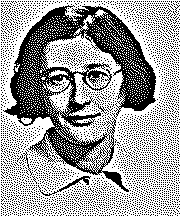
\includegraphics{psimone-retdit.png}}&
	\href{z-psimone-retditR2.png}{\includegraphics{psimone-retditR2.png}}&
	\href{z-psimone-retditZ2.png}{\includegraphics{psimone-retditZ2.png}}\\
	input & random & zeros
\end{tabular}

\section{Implementation}

A C implementation of this technique is available in
\href{https://github.com/mnhrdt/imscript/blob/master/src/mdither.c}{imscript},
as the program~\verb+mdither+.  All the experiments described in this page
have been created automatically by extracting the comments in the source (see
the HTML source to view them).


\subsection{Floyd-Sternberg dithering}

To binarize a gray-scale image by Floyd-Sternberg dithering you can use the
program ``\verb+dither+''

%RUN_VERBATIMS sh
\begin{verbatim}
dither i/weil.png weil-dit.png
\end{verbatim}
\begin{tabular}{cc}
	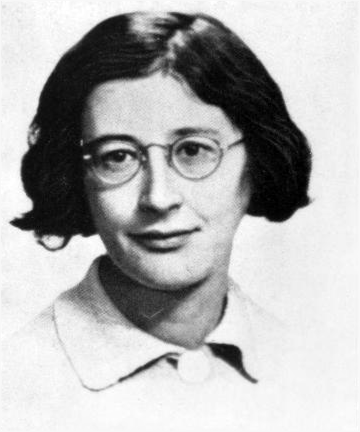
\includegraphics{i/weil.png} &
	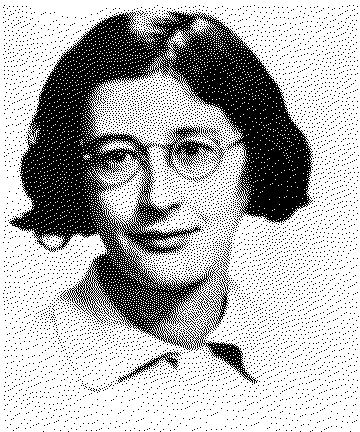
\includegraphics{weil-dit.png} \\
	\verb+weil.png+ &
	\verb+weil-dit.png+
\end{tabular}

\subsection{Counting the carrying capacity of an image}

The program ``\verb+mdither count+'' prints the number of bits, bytes, kilobites
and megabytes that can be potentially encoded on a given image

\begin{verbatim}
mdither count weil-dit.png > weil-capacity.txt
\end{verbatim}
\VerbatimInput{weil-capacity.txt}

\subsection{Encoding bits into a carrier image}

The program ``\verb+mdither encode+'' encodes a stream of bytes into a
carrier image.  In the following example we encode a random stream of bits
and a stream of zeros in the same carrier image.

\begin{verbatim}
mdither encode weil-dit.png weil-random.png /dev/urandom
mdither encode weil-dit.png weil-zeros.png  /dev/zero
\end{verbatim}
\begin{tabular}{cc}
	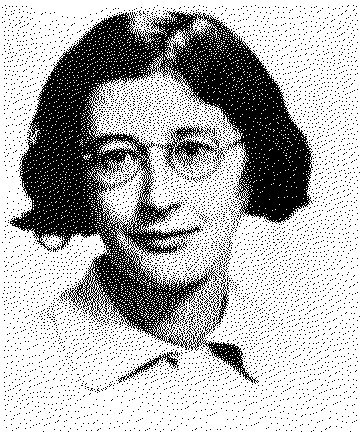
\includegraphics{weil-random.png} &
	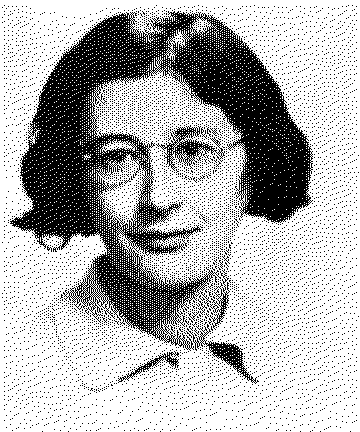
\includegraphics{weil-zeros.png} \\
	\verb+weil-random.png+ &
	\verb+weil-zeros.png+
\end{tabular}

\subsection{Decoding bits from an image}

And this information can be extracted by the program ``\verb+mdither decode+'':
\begin{verbatim}
mdither decode weil-random.png | hexdump -vn 128 > weil-random.txt
mdither decode weil-zeros.png  | hexdump -vn 128 > weil-zeros.txt
\end{verbatim}

Contents of file \verb+weil-random.txt+:
\VerbatimInput{weil-random.txt}

Contents of file \verb+weil-zeros.txt+:
\VerbatimInput{weil-zeros.txt}


\section{Examples}

Here we show examples of random bits encoded into the example images of this
project, using different resolutions.
En each case, we show the binary image along the number of bytes of encoded
information it contains.

In all cases, the images were pre-processed by a linear retinex filter and a
contrast change that forces the background to be a light-gray (in order to
maximize the available space for encoding the information).

%SCRIPT qauto j/i1.png | plambda 'x,l -1 *'|blur -z z 0.1|qauto - photo1.png
%SCRIPT qauto j/i2.png | plambda 'x,l -1 *'|blur -z z 0.1|qauto - photo2.png
%SCRIPT qeasy 10 120 j/i3.png | plambda 'x,l -1 *'|blur -z z 0.1|qauto - photo3.png
%SCRIPT qeasy 30 70 j/i4.png | plambda 'x,l -1 *'|blur -z z 0.1|qauto - photo4.png
%SCRIPT qeasy 40 170 j/i5.png | plambda 'x,l -1 *'|blur -z z 0.1|qauto - photo5.png

%SCRIPT for i in 1 2 3 4 5; do for j in 1 2 3 4 5 6 7; do downsa v $j photo$i.png |qauto| dither - diphoto-${i}-${j}.png ; done ; done

%SCRIPT for i in diphoto*png; do mdither count $i | cut -d' ' -f3 > bytes-$i ; done
%SCRIPT for i in diphoto*png; do mdither2 count $i | cut -d' ' -f3 > bytes2-$i ; done
%SCRIPT for i in diphoto*png; do mdither encode $i E$i /dev/urandom ; done
%SCRIPT for i in diphoto*png; do mdither2 encode $i E2$i /dev/urandom ; done

\subsection{Test image ``photo 1''}
\begin{tabular}{lllllll}
	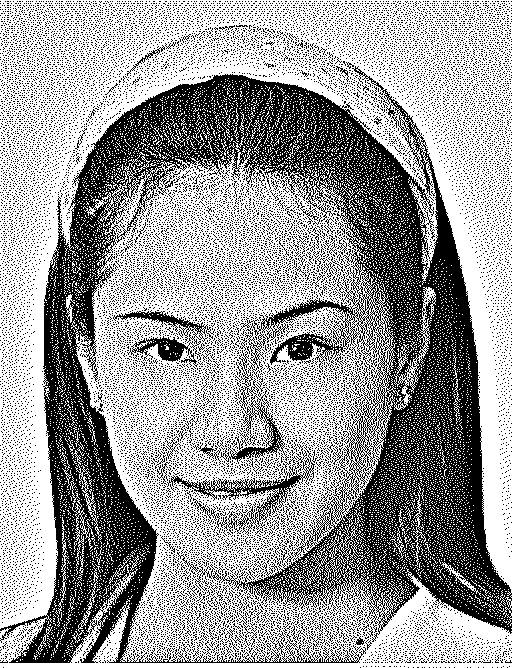
\includegraphics{Ediphoto-1-1.png} &
	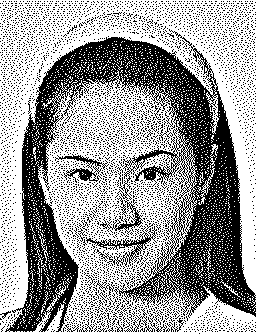
\includegraphics{Ediphoto-1-2.png} &
	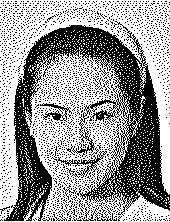
\includegraphics{Ediphoto-1-3.png} &
	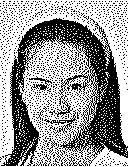
\includegraphics{Ediphoto-1-4.png} &
	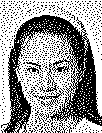
\includegraphics{Ediphoto-1-5.png} &
	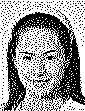
\includegraphics{Ediphoto-1-6.png} &
	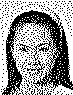
\includegraphics{Ediphoto-1-7.png} \\
	\input{bytes-diphoto-1-1.png} &
	\input{bytes-diphoto-1-2.png} &
	\input{bytes-diphoto-1-3.png} &
	\input{bytes-diphoto-1-4.png} &
	\input{bytes-diphoto-1-5.png} &
	\input{bytes-diphoto-1-6.png} &
	\input{bytes-diphoto-1-7.png} \\
\end{tabular}
\begin{tabular}{lllllll}
	\includegraphics{E2diphoto-1-1.png} &
	\includegraphics{E2diphoto-1-2.png} &
	\includegraphics{E2diphoto-1-3.png} &
	\includegraphics{E2diphoto-1-4.png} &
	\includegraphics{E2diphoto-1-5.png} &
	\includegraphics{E2diphoto-1-6.png} &
	\includegraphics{E2diphoto-1-7.png} \\
	\input{bytes2-diphoto-1-1.png} &
	\input{bytes2-diphoto-1-2.png} &
	\input{bytes2-diphoto-1-3.png} &
	\input{bytes2-diphoto-1-4.png} &
	\input{bytes2-diphoto-1-5.png} &
	\input{bytes2-diphoto-1-6.png} &
	\input{bytes2-diphoto-1-7.png} \\
\end{tabular}

\subsection{Test image ``photo 2''}
\begin{tabular}{lllllll}
	\includegraphics{Ediphoto-2-1.png} &
	\includegraphics{Ediphoto-2-2.png} &
	\includegraphics{Ediphoto-2-3.png} &
	\includegraphics{Ediphoto-2-4.png} &
	\includegraphics{Ediphoto-2-5.png} &
	\includegraphics{Ediphoto-2-6.png} &
	\includegraphics{Ediphoto-2-7.png} \\
	\input{bytes-diphoto-2-1.png} &
	\input{bytes-diphoto-2-2.png} &
	\input{bytes-diphoto-2-3.png} &
	\input{bytes-diphoto-2-4.png} &
	\input{bytes-diphoto-2-5.png} &
	\input{bytes-diphoto-2-6.png} &
	\input{bytes-diphoto-2-7.png} \\
\end{tabular}
\begin{tabular}{lllllll}
	\includegraphics{E2diphoto-2-1.png} &
	\includegraphics{E2diphoto-2-2.png} &
	\includegraphics{E2diphoto-2-3.png} &
	\includegraphics{E2diphoto-2-4.png} &
	\includegraphics{E2diphoto-2-5.png} &
	\includegraphics{E2diphoto-2-6.png} &
	\includegraphics{E2diphoto-2-7.png} \\
	\input{bytes2-diphoto-2-1.png} &
	\input{bytes2-diphoto-2-2.png} &
	\input{bytes2-diphoto-2-3.png} &
	\input{bytes2-diphoto-2-4.png} &
	\input{bytes2-diphoto-2-5.png} &
	\input{bytes2-diphoto-2-6.png} &
	\input{bytes2-diphoto-2-7.png} \\
\end{tabular}


\subsection{Test image ``photo 3''}
\begin{tabular}{lllllll}
	\includegraphics{Ediphoto-3-1.png} &
	\includegraphics{Ediphoto-3-2.png} &
	\includegraphics{Ediphoto-3-3.png} &
	\includegraphics{Ediphoto-3-4.png} &
	\includegraphics{Ediphoto-3-5.png} &
	\includegraphics{Ediphoto-3-6.png} &
	\includegraphics{Ediphoto-3-7.png} \\
	\input{bytes-diphoto-3-1.png} &
	\input{bytes-diphoto-3-2.png} &
	\input{bytes-diphoto-3-3.png} &
	\input{bytes-diphoto-3-4.png} &
	\input{bytes-diphoto-3-5.png} &
	\input{bytes-diphoto-3-6.png} &
	\input{bytes-diphoto-3-7.png} \\
\end{tabular}
\begin{tabular}{lllllll}
	\includegraphics{E2diphoto-3-1.png} &
	\includegraphics{E2diphoto-3-2.png} &
	\includegraphics{E2diphoto-3-3.png} &
	\includegraphics{E2diphoto-3-4.png} &
	\includegraphics{E2diphoto-3-5.png} &
	\includegraphics{E2diphoto-3-6.png} &
	\includegraphics{E2diphoto-3-7.png} \\
	\input{bytes2-diphoto-3-1.png} &
	\input{bytes2-diphoto-3-2.png} &
	\input{bytes2-diphoto-3-3.png} &
	\input{bytes2-diphoto-3-4.png} &
	\input{bytes2-diphoto-3-5.png} &
	\input{bytes2-diphoto-3-6.png} &
	\input{bytes2-diphoto-3-7.png} \\
\end{tabular}

\subsection{Test image ``photo 4''}
\begin{tabular}{lllllll}
	\includegraphics{Ediphoto-4-1.png} &
	\includegraphics{Ediphoto-4-2.png} &
	\includegraphics{Ediphoto-4-3.png} &
	\includegraphics{Ediphoto-4-4.png} &
	\includegraphics{Ediphoto-4-5.png} &
	\includegraphics{Ediphoto-4-6.png} &
	\includegraphics{Ediphoto-4-7.png} \\
	\input{bytes-diphoto-4-1.png} &
	\input{bytes-diphoto-4-2.png} &
	\input{bytes-diphoto-4-3.png} &
	\input{bytes-diphoto-4-4.png} &
	\input{bytes-diphoto-4-5.png} &
	\input{bytes-diphoto-4-6.png} &
	\input{bytes-diphoto-4-7.png} \\
\end{tabular}
\begin{tabular}{lllllll}
	\includegraphics{E2diphoto-4-1.png} &
	\includegraphics{E2diphoto-4-2.png} &
	\includegraphics{E2diphoto-4-3.png} &
	\includegraphics{E2diphoto-4-4.png} &
	\includegraphics{E2diphoto-4-5.png} &
	\includegraphics{E2diphoto-4-6.png} &
	\includegraphics{E2diphoto-4-7.png} \\
	\input{bytes2-diphoto-4-1.png} &
	\input{bytes2-diphoto-4-2.png} &
	\input{bytes2-diphoto-4-3.png} &
	\input{bytes2-diphoto-4-4.png} &
	\input{bytes2-diphoto-4-5.png} &
	\input{bytes2-diphoto-4-6.png} &
	\input{bytes2-diphoto-4-7.png} \\
\end{tabular}

\subsection{Test image ``photo 5''}
\begin{tabular}{lllllll}
	\includegraphics{Ediphoto-5-1.png} &
	\includegraphics{Ediphoto-5-2.png} &
	\includegraphics{Ediphoto-5-3.png} &
	\includegraphics{Ediphoto-5-4.png} &
	\includegraphics{Ediphoto-5-5.png} &
	\includegraphics{Ediphoto-5-6.png} &
	\includegraphics{Ediphoto-5-7.png} \\
	\input{bytes-diphoto-5-1.png} &
	\input{bytes-diphoto-5-2.png} &
	\input{bytes-diphoto-5-3.png} &
	\input{bytes-diphoto-5-4.png} &
	\input{bytes-diphoto-5-5.png} &
	\input{bytes-diphoto-5-6.png} &
	\input{bytes-diphoto-5-7.png} \\
\end{tabular}
\begin{tabular}{lllllll}
	\includegraphics{E2diphoto-5-1.png} &
	\includegraphics{E2diphoto-5-2.png} &
	\includegraphics{E2diphoto-5-3.png} &
	\includegraphics{E2diphoto-5-4.png} &
	\includegraphics{E2diphoto-5-5.png} &
	\includegraphics{E2diphoto-5-6.png} &
	\includegraphics{E2diphoto-5-7.png} \\
	\input{bytes2-diphoto-5-1.png} &
	\input{bytes2-diphoto-5-2.png} &
	\input{bytes2-diphoto-5-3.png} &
	\input{bytes2-diphoto-5-4.png} &
	\input{bytes2-diphoto-5-5.png} &
	\input{bytes2-diphoto-5-6.png} &
	\input{bytes2-diphoto-5-7.png} \\
\end{tabular}


\section{Conclusion and ongoing work}

This note shows that a simple criterion suffices to encode a \emph{linear
amount of bits} into dithered binary images \emph{without noticeable loss in
visual quality}.  The method achieves an average~$25\%$ efficiency (1/4 bits
per pixel) for images without saturated regions.

Most of the improvements can be obtained by changing the table of patterns.

Here are some possible improvements:

\begin{enumerate}
	\item Improve the efficiency to~$50\%$.  This is a very low-hanging
		fruit.  It suffices to change slightly the table of patterns
		so that the three groups of patterns of the same intensity
		belong to the same group, then we can encode 2 bits on each,
		effectively duplicating the available information content.
	\item Improve the efficiency to near~$100\%$.  Of course
		full-efficiency is impossible because all the information
		would be used for the encoding and none would be available
		for the carrier image.  But we can easily have a much higher
		rate by using a table of patterns with larger cells.  For
		example, by using cells of size~$3\times3$, there are~$512$
		possible cells, and their intensities, between 0 and 9, are
		arranged in groups according to the 9th line of pascal
		triangle
		$$
		1\ 9\ 36\ 79\ 102\ 102\ 79\ 36\ 9\ 1
		$$
		Now, by conflating the three central intensities, we have
		more than $2^8$ possible cells, and we can encode 8 bits of
		information on their choice, thus reaching an information
		content of~$8/9=88.9\%$ on these cells, and about~$75\%$ on
		average (assuming a uniform distribution of the possible
		cells).  By using larger cells it is clear than we can
		get a theoretical efficiency as high as we want (at the
		price of final image resolution).
	\item So far we have assumed that cells of the same average intensity
		can be interchanged with negligible information loss.
		However, this is a gross simplification.  For example, in the
		following table
		\begin{tabular}{llll}
			\includegraphics{pat4_a.png} &
			\includegraphics{pat4_b.png} &
			\includegraphics{pat4_c.png} &
			\includegraphics{pat4_d.png} \\
			A & B & C & D
		\end{tabular}
		the $4\times4$ cells A and B can be probably identified
		without loss of visual information, but changing between C
		and D will have a greater visual impact.  This means that
		cells of the same intensity are not necessarily equivalent,
		and by carefully building the table of patterns we may obtain
		much better results for a given carrying capacity.
	\item In the light of the previous observation, it might be
		interesting to build the table of patterns as the optimum of
		a variational criterion that minimizes visual loss while
		achieving an optimum carrying capacity.  Notice that this
		algorithm can be very expensive to run, but only upon the
		creation of the table.  Once the table is decided, encoding
		and decoding are fast, real-time operations.  This will
		surely produce better tables than hand-crafted ones.
\end{enumerate}
%SCRIPT printf 'P2\n4 4\n1\n0 1 0 1\n1 0 1 0\n0 1 0 1\n1 0 1 0\n'|plambda '200 *'|ntiply 16 - pat4_a.png
%SCRIPT printf 'P2\n4 4\n1\n1 0 1 0\n0 1 0 1\n1 0 1 0\n0 1 0 1\n'|plambda '200 *'|ntiply 16 - pat4_b.png
%SCRIPT printf 'P2\n4 4\n1\n1 1 1 1\n1 1 1 1\n0 0 0 0\n0 0 0 0\n'|plambda '200 *'|ntiply 16 - pat4_c.png
%SCRIPT printf 'P2\n4 4\n1\n1 1 0 0\n1 1 0 0\n1 1 0 0\n1 1 0 0\n'|plambda '200 *'|ntiply 16 - pat4_d.png

% vim:set tw=77 filetype=tex spell spelllang=en:
